\documentclass[a4paper, oneside, 11pt]{article}
%% -> Für längere Arbeiten "report" benutzen.

%% --------------------------------------------------------------------- %%

\usepackage{ifthen}
\newboolean{english}
% \setboolean{english}{true} %% -> Kommentar entfernen bei englischen Arbeiten

%% --------------------------------------------------------------------- %%

%% -> Einfügen der Definitionen
%% -> Deutsche Anpassung 
\usepackage[T1]{fontenc}
\usepackage[ngerman,english]{babel}
%\usepackage{babelbib}
\usepackage{ifthen}
%% --------------------------------------------------------------------- %%

%% -> Farben einfügen
\usepackage{color}
\usepackage{xcolor}

% -> Definierte Farben
\definecolor{MSBlue}{rgb}{.204,.353,.541} 
\definecolor{trueblue}{rgb}{0.0, 0.45, 0.81}
\definecolor{onyx}{rgb}{0.06, 0.06, 0.06}
\definecolor{mygruen}{rgb}{0.4660, 0.6740, 0.1880}
\definecolor{plotblue}{rgb}{0, 0.4470, 0.7410}
\definecolor{myrot}{rgb}{0.8500, 0.3250, 0.0980}
\definecolor{mygreen}{RGB}{28,172,0} %% Matlab Kommentar
\definecolor{mylilas}{RGB}{170,55,241} %% Matlab String

%% --------------------------------------------------------------------- %%

%% -> Grafiken 
\usepackage{graphicx}
\usepackage{epstopdf}
\usepackage{wallpaper}
\usepackage{float} %% Verbessert die Platzierung
%% --------------------------------------------------------------------- %%

\usepackage[tmargin=1in,bmargin=1in,lmargin=1.25in,rmargin=1.25in]{geometry}
\setlength{\parindent}{0em}
\setlength{\parskip}{1.5ex plus0.5ex minus0.5ex}
\usepackage{setspace}
\onehalfspacing

\usepackage{pst-all} %% erweiterte Zeichenbefehle

%% -> Schriftart
\usepackage{helvet}
\renewcommand{\familydefault}{phv}

%% -> Layout Überprüfung
\usepackage{layout}
\usepackage{xspace}

%% -> Für Tabellen
\usepackage{array}
\usepackage{booktabs}
\usepackage{dcolumn}
\usepackage{multirow}

%% -> Einrücken von und Abstand zwischen Absätzen
\setlength{\parindent}{0em}
\setlength{\parskip}{1.5ex plus0.5ex minus0.5ex}

%% -> Tabulator Funktion
\newcommand\tab[1][1cm]{\hspace*{#1}}

%% -> Weniger Warnungen wegen überfüllter Boxen
\tolerance = 9999
\sloppy

%% -> Erweiterte Einstellungen der Bildunterschriften bzw. Tabellenunterschriften
\usepackage{caption}
\usepackage{subcaption}
\captionsetup[figure]{labelfont=footnotesize, textfont=footnotesize}
\captionsetup[table]{labelfont=footnotesize, textfont=footnotesize}

%% -> Hyperref
%\usepackage[pdftex,bookmarks=true,bookmarksnumbered=true,]{hyperref}

\usepackage[hidelinks]{hyperref}
% \usepackage[colorlinks=true]{hyperref}
% \hypersetup{
% colorlinks=true,
% linkbordercolor={1 0 0},
% citebordercolor={0 1 0},
% filebordercolor={1 0 1},
% runbordercolor={1 0 1},
% urlbordercolor={0 0 1},
% }

%% -> Quellen
\usepackage[super, square, sort&compress]{natbib}

%%-> Weitere nützliche Pakete
\usepackage{todonotes}
\setlength {\marginparwidth }{2cm}
%% --------------------------------------------------------------------- %%

% -> Für Codes zum einfügen
\usepackage{listings}
%\lstset{numbers=left,numberstyle=\tiny,stepnumber=5,numbersep=5pt}

%% -> Für MATLAB Code
\lstset
{language=Matlab,%
    basicstyle=\scriptsize,
    breaklines=true,%
    captionpos=b,
    frame = single,
    morekeywords={matlab2tikz},
    keywordstyle=\color{blue},%
    morekeywords=[2]{1}, keywordstyle=[2]{\color{black}},
    identifierstyle=\color{black},%
    stringstyle=\color{mylilas},
    commentstyle=\color{mygreen},%
    showstringspaces=false,%
    %numbers=left,%
    %numberstyle={\footnotesize \color{black}},%
    %stepnumber=5, %
    %numbersep=9pt, % 
    emph=[1]{for,end,break},emphstyle=[1]\color{red}, %
    emph=[2]{all}, emphstyle=[2]\color{mylilas},    
}
%% --------------------------------------------------------------------- %%

% -> Kopf und Fußzeile gestallten
\usepackage{fancyhdr}
%\setlength{\headheight}{13.6pt}
\setlength{\footskip}{41pt}
\rhead{} 
\chead{} 
\lhead{}
\renewcommand{\headrulewidth}{0pt}
\lfoot{
\includegraphics[width=\textwidth*1/6]{Definition/DUH-positive.eps}}
\rfoot{\small\thepage}
\cfoot{}
\renewcommand{\footrulewidth}{0pt}
%% --------------------------------------------------------------------- %%

%% -> Matematische Packages
\usepackage{amsmath,amssymb,amsfonts,amstext}
\usepackage{mathtools}
\usepackage{mathrsfs}

%% -> SI-Einheiten
%\usepackage{units}
\usepackage{siunitx}
% \usepackage{physics}
\sisetup{locale = DE,separate-uncertainty}
\sisetup{list-final-separator={ und }}
\sisetup{per-mode=fraction}
\DeclareSIUnit\Pascal{\newton\per\square\metre}
%\sisetup{output-decimal-marker = {.}} %% Für Punkttrennung nur bei englischen Arbeiten erforderlich
%% --------------------------------------------------------------------- %%

%% -> Für die Überschriften
\usepackage{titlesec}
\titleformat{\section}{\LARGE\sffamily\bfseries}{\thesection}{1em}{}
\titleformat{\subsection}{\Large\bfseries\sffamily}{\thesubsection}{1em}{}
\titleformat{\subsubsection}{\large\sffamily\bfseries}{\thesubsubsection}{1em}{}
%% --------------------------------------------------------------------- %%

%% -> Bildnummerierung ist logisch mit Kapitelnummerierung
\numberwithin{figure}{section}
\numberwithin{table}{section}
\numberwithin{equation}{section}
%\numberwithin{equation}{subsection}
%% --------------------------------------------------------------------- %%

%% -> Schaltplan zeichnen und Grafiken und für PGF Plots
\usepackage[european, siunitx]{circuitikz}
\usetikzlibrary{circuits.ee.IEC}
\usepackage{tikz}
\usepackage{tikzscale}
\usepackage{pgfplots}
\pgfplotsset{compat=1.4}
\newlength\figH
\newlength\figW
\setlength{\figH}{6cm}
\setlength{\figW}{8cm}
%% --------------------------------------------------------------------- %%

%% -> Für Vektoren
\usepackage{amsmath}

% For pie-charts
\usepackage{amsmath,amssymb,amsfonts,amstext}
\usepackage{mathtools}
\usepackage{mathrsfs}
\usepackage{pgf-pie}

%% -> Deckblatt ausfüllen 
\def\labtitle{Strategisches Marketing}
\def\labcode{MECH-M-2-MSK-STM-SE}
\def\labname{Markenanalyse zu Garmin Sportuhren}
\def\labnum{Berichtnummer}
\def\study{Master Mechatronik and Smart Technologies}
\def\branch{}
\def\term{2.}
\def\lecturer{Maria Wallhöfer}
\def\group{MA-MECH-23-BB}
\def\student{Abfalterer, Figl, Posch}

%% --------------------------------------------------------------------- %%

%% -> Beginn des Dokumentes

\begin{document}
\newcounter{romanPagenumber}

%% -> Sprache auswählen
\ifthenelse{\boolean{english}}{\selectlanguage{english}}{\selectlanguage{ngerman}}
\selectlanguage{ngerman}
%\selectlanguage{english}

%% -> Fußzeile und Kopfzeile einfügen
\pagestyle{fancy}

\pagenumbering{Roman}
%% -> Deckblatt laden
%% Deckblatt %%

\thispagestyle{empty}
\sffamily
\ThisTileWallPaper{\paperwidth}{\paperheight}{Deckblatt/MCIHintergrundKPL.pdf}

\vspace*{1cm}
\def\thesis{\ifthenelse{\boolean{english}}{Projekt Report}{Projektbericht}}
\textcolor{MSBlue}{\rmfamily\bfseries\Huge\thesis}

\vspace*{0.5cm}
\textbf{\labtitle{}(\labcode)}

\textbf{\labname}

% \ifthenelse{\boolean{english}}{\textbf{Report} }{\textbf{Labor }}\textbf{\labnum}


\vspace*{13cm}

\textcolor{gray}{\study}

% \def\studybranch{\ifthenelse{\boolean{english}}{Study Branch}{Studienzweig}}
% \textcolor{gray}{\studybranch: \branch}

\def\termname{\ifthenelse{\boolean{english}}{semester}{Semester}}
\textcolor{gray}{\term{ }\termname}

\def\lecturername{\ifthenelse{\boolean{english}}{Responsible lecturer}{Lehrveranstaltungsleiter}}
\textcolor{gray}{\lecturername: \lecturer}

\def\groupname{\ifthenelse{\boolean{english}}{Group}{Jahrgang}}
\textcolor{gray}{\groupname: \group}

\def\authorname{\ifthenelse{\boolean{english}}{Author}{Verfasser}}
\textcolor{gray}{\authorname: \student}

\textcolor{gray}{\today}

\newpage

\setcounter{romanPagenumber}{\value{page}}

%% -> Inhaltsverzeichnis
\tableofcontents%\thispagestyle{empty}
\clearpage

\pagestyle{fancy}
\pagenumbering{arabic}
% =============================================================================
\section{Garmin Sportuhren} \label{sec:garmin}
Garmin ist eine bekannte Marke im Bereich der Sportuhren und hat sich auch einen Namen im Bereich der GPS-Geräte gemacht. Die Firma und deren Produkte zeichnen sich durch ihre Innovationskraft, Zuverlässigkeit und Qualität aus. Die wichtigsten Punkte der Marke Garmin in Bezug auf Marketing können wie folgt aufgelistet werden:

\begin{enumerate}
    \item \textbf{Markenimage und Positionierung} \\
    Garmin hat sich als eine der führenden Marken für GPS-Technologie und Wearables etabliert. Die Marke ist für ihre hochwertigen Produkte und ihre Zuverlässigkeit bekannt, insbesondere im Bereich Sportuhren und Outdoor.

    \item \textbf{Produktvielfalt und Zielgruppen} \\
    Garmin bietet eine breite Palette von Sportuhren für verschiedene Zielgruppen an, darunter Profisportler, Fitness-Enthusiasten und Outdoor-Abenteurer. Die Produkte werden entwickelt, um den individuellen Bedürfnissen und Anforderungen verschiedener Sportarten und Sportlern gerecht zu werden.

    \item \textbf{Innovationsführerschaft} \\
    Garmin ist bekannt für seine kontinuierliche Innovation und die Integration neuer Technologien in seine Produkte. Dazu gehören fortgeschrittene GPS- und Herzfrequenzmessung, Fitness-Tracking und Trainingsanalysen.

    \item \textbf{Marketingstrategien} \\
    Garmin nutzt verschiedene Marketingkanäle, um für seine Produkte zu werben und seine Zielgruppen zu erreichen. Dazu gehören Online-Werbung, Social-Media-Marketing, Influencer-Marketing, Partnerschaften mit Sportveranstaltungen sowie Präsenz in Sportgeschäften und Messen.

    \item \textbf{Kundenerfahrung und Community-Engagement} \\
    Garmin legt Wert auf die Kundenerfahrung und bietet einen umfassenden Kundensupport sowie Community-Plattformen für den Austausch von Erfahrungen und Tipps unter den Nutzern seiner Produkte.

    \item \textbf{Markenloyalität und Reputation} \\
    Durch seine Qualität, Zuverlässigkeit und Kundenzufriedenheit hat sich Garmin eine starke Markenloyalität und eine positive Reputation in der Community aufgebaut.    
\end{enumerate}

Insgesamt ist Garmin eine Marke, die durch ihre technologische Exzellenz, ihr breites Produktsortiment und ihre starke Kundenorientierung im Bereich Sportuhren und GPS-Geräte herausragt. Ihre Marketingstrategien zielen darauf ab die Marke als führende Wahl für Sportler und Outdoor-Enthusiasten zu positionieren.

\newpage
\section{Kundenbefragung} \label{sec:befragung}

Um zunächst die Markenpositionierung von Garmin zu ermitteln ist es notwendig eine Kundenbefragung durchzuführen. Mithilfe der Antworten dieser Umfrage ist es möglich einen ungefähren Überblick zur Markenpositionierung von Garmin zu finden. Der Fragebogen und die Antworten sind jeweils im Anhang (\ref{tab:fragebogen}, \ref{tab:kunden}) zu finden. Es sollte jedoch bedacht werden, dass aufgrund der limitierten Anzahl an befragten Personen, nur ein grober Überblick geschafft wird.

\subsection{Top of Mind Awareness}
Die Top of Mind Awareness  ist ein Begriff der Markenbekanntheit und beschreibt welche Marke Personen als erstes für eine bestimmte Kategorie einfällt. Sprich mit welchem Produkt als erstes eine Assoziation zu einer Produktkategorie geknüpft wird. Die Top of Mind Awareness ist ein essentieller Bestandteil bei Kaufentscheidungen von potentiellen Kunden und deshalb auch ein sehr wichtiges Kriterium zur Bewertung der Stärke einer Marke. Die Agreggierung von Neukunden wird durch die Top of Mind Awareness auch viel leichter, da die Marke bei Recherchen bzw. Gesprächen viel schneller in den Vordergrund rückt. Ist die Marke aufgrund von z.B. Skandalen bei vielen Kunden im Kopf, kann die Top of Mind Awareness jedoch auch negativ sein.  \cite{ToMA-1} \cite{ToMA-2}

Anhand der Befragung \ref{sec:befragung} lässt sich leicht feststellen, dass Garmin eine sehr hohe Top of Mind Awaraness bei Sportuhren besitzt, da jeder befragte als erste Marke Garmin aufgezählt hat. In Abbildung \ref{fig:toMa} ist dies nochmals grafisch zu sehen, dabei ist zu beachten, dass manche Personen 2 Marken gewählt haben. 


\begin{figure}[H]
    \centering
    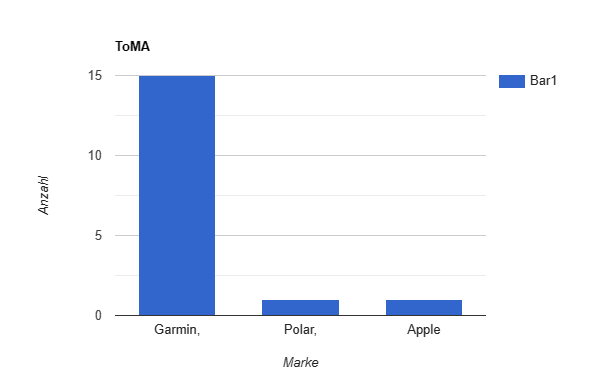
\includegraphics[width=0.7\linewidth]{Figure/ToMA.png}
    \caption{Garmin - Top of Mind Awaraness}
    \label{fig:toMa}
\end{figure}


Es sollten jedoch keine voreiligen Schlüsse gezogen werden, da die befragten Personen bereits alle Garmin Uhren besitzen und im alltäglichen Gebrauch verwenden. Zudem konnten alle Personen noch einige weitere Marken nennen. Um eine genauerer Positionierung zu ermitteln, müsste eine viel größere Anzahl an Personen befragt werden und auch eine weniger homogene Gruppe befragt werden.

\subsection{Involvement}
Bei Marketing spricht man bei Involvement meist bei Entscheidungs- bzw. Kaufsituationen. Involvement beschreibt grundlegend wie viel Zeit und Energie Kunden in die Suche und Bewertung von Produkten investieren. Dabei lassen sich Käufe grob in zwei Kategorien einteilen.
\begin{itemize}
    \item \textbf{High-Involvement:} Die Kaufentscheidung wird durch eine intensive Recherche und viele Vergleiche zwischen verschiedenen Produkten getätigt. Dabei handelt es sich bei High-Involvement Käufen meist um eher teurere Anschaffungen, wie z.B. eine Uhr oder ein Auto. In der High-Involvement Kategorie spielt die stärke einer Marke eine essentielle Rolle damit der Kunde ein Gefühl von Sicherheit erhält. Damit sind diese Käufe auch stark mit der Top of Mind Awareness verknüpft.
    \item \textbf{Low-Involvement:}
    Die Kaufentscheidung wird meist unterbewusst und ohne lange Recherche getätigt. Dabei handelt es sich meist um eher billigere Produkte, wie z.B. Waschmittel. Die stärke einer Marke ist hier nicht unbedingt ausschlaggebend. \cite{Involvement-1} \cite{Involvement-2}
\end{itemize}

Sportuhren fallen aufgrund des nicht so geringen Preis eher in die Kategorie von High-Involvement Gegenständen. Das ist auch bei Garmin Uhren so und ist anhand der Befragung \ref{sec:befragung} sehr einfach ersichtlich. Nahezu alle befragten haben vor dem Kauf der Uhr recherchiert und vergleiche zwischen verschiedenen Marken durchgeführt bevor es zu einem Kauf gekommen ist. In den Abbildungen (\ref{fig:inv1}, \ref{fig:inv2}) ist zu sehen ob sich die Befragten zuvor informiert haben und auch ob sie das Produkt Online oder im Geschäft gekauft haben.

\begin{figure}[!h]
  \centering
  \begin{minipage}[b]{0.48\textwidth}
    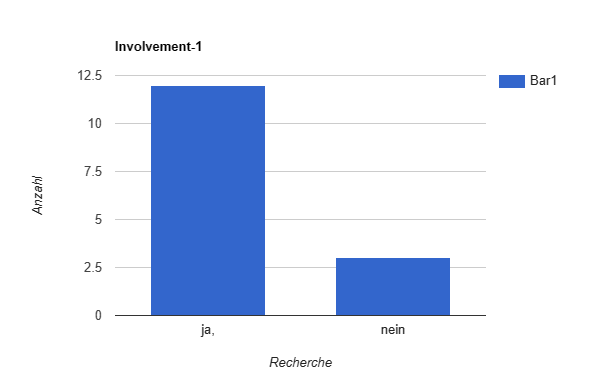
\includegraphics[width=\textwidth]{Figure/involvement-1.png}
      \caption{Garmin - Involvement}
    \label{fig:inv1}
  \end{minipage}
  \hfill
  \begin{minipage}[b]{0.48\textwidth}
    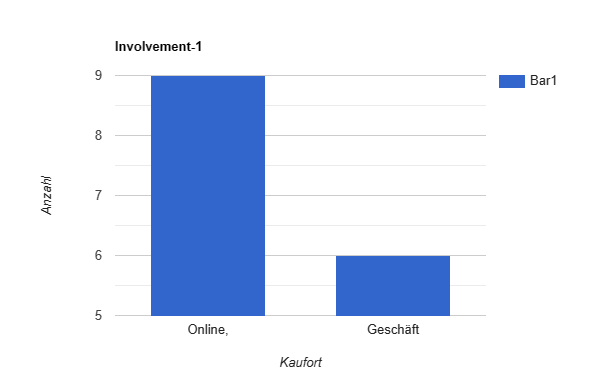
\includegraphics[width=\textwidth]{Figure/involvement-2.png}
    \caption{Garmin - Kaufort}
    \label{fig:inv2}
  \end{minipage}
\end{figure}




\newpage


% Luki
\subsection{Bewertungskriterien}
Die Befragten stützen sich auf verschiedene Merkmalen beim Vergleich von Garmin mit anderen Marken. Einige der hervorgehobenen Merkmale sind die Funktionsvielfalt, Genauigkeit der Daten, Benutzerfreundlichkeit der Geräte, und die Optik der Uhren. Im Zuge dieser Umfrage wurde auch schnell klar, dass sich Garmin bereits einen starken Namen in der gesamten Sport Gemeinschaft gemacht hat und alleine durch Image und Mundpropaganda einen großen Kundenkreis schafft. 

In Bezug auf den Nutzen, den Garmin-Produkte für die Befragten schaffen, wurde eine Reihe von Aspekten hervorgehoben. Dazu gehören die Unterstützung vieler verschiedener Sportarten, die Qualität der Trainingsdaten und bereitgestellten Metriken sowie die Robustheit und Akkulaufzeit der Geräte. Diese Aspekte deuten auf einen hohen funktionalen Nutzen hin. Darüber hinaus scheint Garmin auch einen emotionalen Nutzen zu bieten, da die Befragten ihre Geräte sowohl beim Sport als auch im Alltag als ständigen Begleiter dabei haben.

\subsection{Wettbewerbsvorteile}
Die Befragten nehmen Garmin in Bezug auf mehrere kaufentscheidende Merkmale als höherwertig wahr als seine Konkurrenten. Insbesondere wurde die Software und das soziale Netzwerk von Garmin sowie der Funktionsumfang und die Metriken als Unterscheidungsmerkmale hervorgehoben. Darüber hinaus wurde die große Auswahl an Modellen, die Funktionsvielfalt und die Robustheit der Garmin-Produkte als Wettbewerbsvorteile angesehen.

Es ist auch bemerkenswert, dass die Befragten Garmin als Anbieter von hochwertigen Produkten wahrnehmen. Dies deutet darauf hin, dass die Marke in Bezug auf die Produktqualität einen starken Wettbewerbsvorteil hat. Schließlich wurde die Fähigkeit von Garmin, viele Metriken über den Fortschritt zu liefern, als ein weiteres Unterscheidungsmerkmal genannt, das Garmin von seinen Konkurrenten abhebt.

Zusammenfassend lässt sich sagen, dass die Befragten Garmin in Bezug auf eine Reihe von Merkmalen positiv bewerten und die Marke als wertvoll für ihre sportlichen und alltäglichen Aktivitäten ansehen. Dies deutet darauf hin, dass Garmin eine starke Position im Markt für Sport- und Outdooruhren hat.


\newpage


% Mathias
\subsection{Markenimage}
Das Markenimage bezieht sich auf die Wahrnehmung und Vorstellung die Kunden von einem Unternehmen besitzen. Es bildet sich aus verschiedenen Komponenten wie Werbung, Produkterfahrung und der wahrgenommenen Qualität. Dabei führt ein positives Markenimage zu einer hohen Kundenloyalität und stärkt die Marktposition eines Unternehmens.\cite{Markenimage}  
Anhand der Antworten in der Kundenbefragung ist eine klare Tendenz erkennbar, denn die Kunden assoziieren die Produkte der Marke Garmin vor allem mit folgenden Eigenschaften:
\begin{itemize}
    \item Robustheit
    \item Genauigkeit
    \item Funktionsvielfalt
    \item Kompatibilität
\end{itemize} 
Dies führt dazu, dass die Marke im Allgemeinen sehr positiv wahrgenommen wird. Dies deckt sich auch mit den Antworten bezüglich dem Wettbewerbsvorteil, denn auch hier geben die Befragten meist Antworten die sich auf die Qualität der Garmin Produkte beziehen.
Man kann also festhalten, dass sich Garmin seinen Stärken bewusst ist und diese gezielt nutzt, da diese den Kunden beeindrucken und den Kundennutzen darstellen und somit das Markenimage bilden. Denn die positiven Erlebnisse die der Kunde mit den Produkten von Garmin hat, ergeben schlussendlich das Markenimage. Dies deckt sich auch mit den Ergebnissen bezüglich der ungestützen Markenbekanntheit. Hier haben die Befragten stets Garmin genannt, was von einer großen Bekanntheit zeugt, was wiederum die Vorraussetzung für ein gutes Markenimage bildet. 

\subsection{Net Promoter Score (NPS)}

Der Net Promoter Score (NPS) wird verwendet, um die Loyalität und Zufriedenheit von Kunden mit einem Unternehmen zu messen.Um dies messen zu können wird eine einfache Frage gestellt: "Wie wahrscheinlich ist es das sie Ihr Garmin Gerät weiterempfehlen würden? (1: unwahrscheinlich; 10: sehr wahrscheinlich)". Anschließend werden die Kunden je nach Antwort eingestuft, wobei es drei Kategorien von Kunden gibt:
\begin{itemize}
    \item Promotoren (9-10)
    \item Passive (7-8)
    \item Kritiker (0-6)
\end{itemize}
Die Anzahl der Kritiker in Prozent wird dann von der Anzahl der Promotoren in Prozent abgezogen und das Ergebnis ist dann der Net Promoter Score. Das Ergebnis der Kundenberfragung zu Garmin ergibt einen NPS von circa 67. Dieses Ergebnis ist in Abbildung \ref{fig:NPS} veranschaulicht. Es ist zu erkennen, dass es keine Kritiker gibt, das heißt es waren alle Kunden zufrieden. Der NPS ist sehr hoch, was für eine sehr hohe Kundenzufriedenheit spricht, und beweist die Kundenorientierung des Unternehmens. \cite{Netigate-NPS} 

\begin{figure}[h]
	\centering
	\begin{tikzpicture}
    \pie[pos ={8,0},
    radius=2,
    text=legend,
    color={cyan,blue}]
    {33.3 / Passive , 66.7 / Promoter} 
    \end{tikzpicture}
    \vspace{0.5cm}
	\caption{Garmin - Net Promoter Score}
    \label{fig:NPS}
\end{figure}

Diesen sehr guten NPS nutzt Garmin indem die gesamte Produktpalette unter einer Marke verkauft und beworben wird, wie in Kapitel \ref{Markenarchitektur} beschrieben. Dies gibt dem Unternehmen die Möglichkeit, die positiven Kundenerfahrungen und somit auch das Markenimage von einem Produkt auf das nächste zu übertragen. 


\newpage
% Noah
\section{Markenanalyse} \label{sec:markenanalyse}

\subsection{Branding}
Garmin ist bekannt für seine Sportuhren, die eine klare visuelle Identität aufweisen. Ein charakteristisches Merkmal ist das Logo von Garmin selbst, das in der Regel auf den Uhren präsent ist. Das Logo besteht aus einer stilisierten schwarzen Schrift auf einem weißen Hintergrund, was eine gewisse Seriosität und Zuverlässigkeit vermittelt. Das blaue Dreieck steht für Erfolg, Wachstum und Entwicklung wobei der Blauton Zuverlässigkeit und Stabilität demonstriert. \cite{logo}

\begin{figure}[H]
    \centering
    
\includegraphics[width=0.6\linewidth]{Figure/logo.png}
    \caption{Garmin Logo \cite{logo}}
    \label{fig:logo}
\end{figure}

Diese Farbkombination ist einprägsam und sofort mit der Marke verbunden. Zusätzlich sind die Uhren oft in sportlichen Farben wie Schwarz, Rot, oder Blau erhältlich, die Dynamik und Energie ausstrahlen. Symbole und Formen auf den Uhren sind oft funktional, wie zum Beispiel klare Ziffernblätter, intuitive Bedienungsknöpfe und auch grafische Elemente, die Aktivitäten repräsentieren. Diese visuellen Ausdrucksformen tragen dazu bei, dass Garmin-Uhren nicht nur als Sportausrüstung, sondern auch als Modeaccessoire wahrgenommen werden.

\subsection{Markenarchitektur}\label{Markenarchitektur}
Garmin verfolgt im Allgemeinen eine 'Branded House' Strategie, wobei die Hauptmarke Garmin als 'Dachmarke' fungiert und verschiedene Produkte (meist mit Zusammenhang) unter einem Namen anbietet. In diesem Fall umfasst dies nicht nur Sportuhren, sondern auch andere GPS-Produkte wie Navigationsgeräte, Wearables und Outdoor-Geräte. Alle diese Produkte tragen das Garmin-Logo und profitieren von der starken Markenbekanntheit und Reputation, die Garmin aufgebaut hat. Durch diese konsistente Markenführung schafft Garmin Vertrauen bei den Verbrauchern und ermöglicht es ihnen, verschiedene Produkte der Marke mit derselben Qualität und Zuverlässigkeit zu verbinden.

\newpage
% Matthias
\section{Schlussfolgerung} \label{sec:schlulssfolgerung}

Die Ergebnisse aus der Befragung decken sich sehr stark mit den Erkenntnissen der Markenanalyse. Denn beide Methoden ergeben dasselbe Bild, welches zeigt, dass Garmin durch seine Innovation und Qualität glänzt. Dabei hat die Qualität mehrere Aspekte wie Kompatibilität, eine große Community, viele Funktionen, Robustheit und Zuverlässigkeit. Genau diese Aspekte bilden den Wettbewerbsvorteil den Garmin gegenüber seinen Konkurrenten hat. Weiteres überzeugen diese Eigenschaften die Kunden und führen schlussendlich zu einem sehr positiven Markenimage und Net Promoterscore. Dies bewirkt wiederum, dass Nutzer von Garmin Produkten, diese weiterempfehlen und selbst weiter nutzen und auch weitere Produkte von Garmin kaufen werden. Dies ist auch hinsichtlich des High-Involvment Kaufes sehr wichtig, da der Käufer intensiv recherchiert bevor er entscheidet welches Produkt er kauft. Hier provitiert Garmin von den vielen Promotoren die die Marke weiterempfehlen und von dem starken Markenimage. 
% =============================================================================

\clearpage

%% -> Verzeichnisse
\pagestyle{fancy}
\pagenumbering{Roman}
\addtocounter{romanPagenumber}{1}
\setcounter{page}{\theromanPagenumber}

%% --------------------------------------------------------------------- %%

%% -> Literaturverzeichnis IEEE-gerecht
\bibliographystyle{IEEEtran}
\renewcommand\refname{Literaturverzeichnis}
\bibliography{Verzeichnisse/Literatur}
\ifthenelse{\boolean{english}}
{\addcontentsline{toc}{section}{Bibliography}}
{\addcontentsline{toc}{section}{Literaturverzeichnis}}
\newpage
%% --------------------------------------------------------------------- %%

%% -> Abbildungsverzeichnis
\listoffigures
\ifthenelse{\boolean{english}}
{\addcontentsline{toc}{section}{List of Figures}}
{\addcontentsline{toc}{section}{Abbildungsverzeichnis}}
\newpage
%% --------------------------------------------------------------------- %%

%% -> Tabellenverzeichnis
\listoftables 
\ifthenelse{\boolean{english}}{\addcontentsline{toc}{section}{List of Tables}}
{\addcontentsline{toc}{section}{Tabellenverzeichnis}}
\newpage
%% --------------------------------------------------------------------- %%

%% --------------------------------------------------------------------- %%
\clearpage
% -> Anhang
\begin{appendix}
\section{Kundenbefragung}\label{appendix:a}

\subsection{Kunden}
\begin{table}[H]
\caption{Liste der befragten Kunden} \label{tab:kunden}
\begin{center}
\begin{tabular}{ l l l l l l }
\toprule
Kunde       & Geschlecht    & Alter     & Garmin Gerät      & Aktivität     & Intensitätsmin. \\ 
\midrule
Kunde 1     & männlich      & 25        & Forerunner 955 solar          & Radfahren        & 300 \\
Kunde 2     & männlich      & 23        & Forerunner 955 solar          & Radfahren        & 300 \\
Kunde 3     & männlich      & 55        & fenix 6           & Radfahren        & 600 \\
Kunde 4     & weiblich      & 55        & fenix 6           & Krafttraining \& Radfahren        & 400 \\
Kunde 5     & männlich      & 24        & fenix 7           & Laufen \& Krafttraining  & 800 \\

Kunde 6     & männlich      & 35        & Forerunner 945    & Langstreckenlauf      & 300 \\
Kunde 7     & weiblich      & 28        & fenix 6S Pro      & Radfahren             & 200 \\
Kunde 8     & männlich      & 42        & Instinct Solar    & Schwimmen             & 150 \\
Kunde 9     & weiblich      & 38        & Venu Sq           & Wandern               & 180 \\
Kunde 10    & männlich      & 31        & Vivoactive 4      & Triathlon             & 350 \\

Kunde 11    & männlich      & 22        & Forerunner 45     & Laufen                & 1800 \\
Kunde 12    & männlich      & 24        & Vivoactive 4s     & Radfahren             & 300 \\
Kunde 13    & weiblich      & 32        & Forerunner 235    & Laufen                & 150 \\
Kunde 14    & männlich      & 45        & Instinct          & Wandern               & 240 \\
Kunde 15    & männlich      & 28        & Forerunner 945    & Triathlon             & 600 \\
\bottomrule
\end{tabular} 
\end{center}
\end{table} 

\newpage

\subsection{Fragebogen}
\begin{enumerate} \label{tab:fragebogen}
    % 1. Top of mind awareness
    \item Welche Marke kommt Ihnen als ersten in den Sinn für Sport- und Outdooruhren?
    \item Welche weiteren Marken zu diesem Stichwort kennen Sie?
    % 2. Involvement
    \item Warum haben Sie ein Gerät der Marke Garmin gekauft und haben Sie länger über das Produkt recherchiert?
    \item Wo haben Sie ihr Gerät gekauft?
    % 3. Bewertungskriterien
    \item Wo sehen Sie den größten Vorteil von Garminprodukten zur Konkurrenz?
    \item Wo sehen Sie einen Nutzen speziell bei Garmin Produkten?
    % 4. Wettbewerbsvorteil
    \item Glauben Sie das Garmin hochwertige Produkte bietet?
    \item Bei welchen Kriterium hebt sich Garmin von den Konkurrenten ab?
    % 5. Markenimage
    \item Bei welcher Aktivität möchten Sie ihr Garmin Gerät nicht mehr vermissen?
    % 6. Net Promoter Score
    \item Wie wahrscheinlich ist es das sie Ihr Garmin Gerät weiterempfehlen würden? \\
    (1: unwahrscheinlich; 10: sehr wahrscheinlich)
\end{enumerate}

\newpage

\section{Interviews: Kunde 1 bis 5}\label{appendix:b}
\begin{enumerate}
    % 1. Top of mind awareness
    \item Welche Marke kommt Ihnen als ersten in den Sinn für Sport- und Outdooruhren? \\
    Garmin \\
    Garmin \\
    Garmin \\
    Garmin \\
    Garmin
    \item Welche weiteren Marken zu diesem Stichwort kennen Sie? \\
    Suunto, Polar, Xiaomi, Appel \\
    Coros, Polar, Apple, Fitbit \\
    Suunto, Polar, Coros, Apple, Samsung \\
    Suunto, Polar, Coros, Apple, Samsung \\
    Suunto, Polar, Coros
    % 2. Involvement
    \item Warum haben Sie ein Gerät der Marke Garmin gekauft und (haben Sie länger über das Produkt recherchiert)? \\
    weil ich sie wollte, ja  \\
    Bereits bestehender Garmin-Kunde, überzeugt durch Funktion, Optik und Haptik. Ja, längere Recherche und Vergleiche \\
    Robustheit, Genauigkeit und Funktionsvielfalt, Ja \\
    Uhr sowohl für Krafttraining als auch Ausdauersport \\
    Große Vielfalt an Sportarten die unterstützt werden, ja.
    \item Wo haben Sie ihr Gerät gekauft? \\
    Online \\
    Online \\
    im Geschäft \\
    Online \\
    Online
    % 3. Bewertungskriterien
    \item Wo sehen Sie den größten Vorteil von Garminprodukten zur Konkurrenz? \\
    Gleich auf mit Konkurenz \\
    Umfang und Aufbau der Benutzeroberflächen, Optik der Uhren \\
    Vielfalt der Funktionen und der Kompatibilität mit verschiedenem Zubehör \\
    Genauigkeit der Daten und der Benutzerfreundlichkeit der Geräte \\
    Große Vielfalt an Sportarten die unterstützt werden 
    \item Wo sehen Sie einen Nutzen speziell bei Garmin Produkten? \\
    Große Kompatibilität \\
    Erweiterungsmöglichkeiten durch herunterladbare Zusatzfunktionen \\
    Unterstützung vieler verschiedener Sportarten \\
    Planung von Trainingseinheiten und maximierung von Trainingsfortschritt \\
    Effektiveres Training
    % 4. Wettbewerbsvorteil
    \item Glauben Sie das Garmin hochwertige Produkte bietet? \\
    ja \\
    Vergleichbar mit Mitbewerbern \\
    ja \\
    ja \\
    ja
    \item Bei welchen Kriterium hebt sich Garmin von den Konkurrenten ab? \\
    keine Ahnung \\
    Software und Soziales Netzwerk sowie Funktionsumfang \\
    große Auswahl an Modellen, die Funktionsvielfalt, Robustheit \\
    große Auswahl an Funktionen, die hohe Qualität der Produkte \\
    Sehr viele Metriken über Fortschritt
    % 5. Markenimage
    \item Bei welcher Aktivität möchten Sie ihr Garmin Gerät nicht mehr vermissen? \\
    Sport \\
    Im Alltag\\
    Beim Sport \\
    Skitouren \\
    Sport und Alltag
    % 6. Net Promoter Score
    \item Wie wahrscheinlich ist es das sie Ihr Garmin Gerät weiterempfehlen würden? \\
    (1: unwahrscheinlich; 10: sehr wahrscheinlich) \\
    10 \\
    10 \\
    9 \\
    9 \\
    10
\end{enumerate}
\newpage

\section{Interviews: Kunde 6 bis 10}\label{appendix:c}
\begin{enumerate}
    % 1. Top of mind awareness
    \item Welche Marke kommt Ihnen als ersten in den Sinn für Sport- und Outdooruhren? \\
    Garmin \\
    Garmin \\
    Garmin \\
    Garmin \\
    Garmin
    \item Welche weiteren Marken zu diesem Stichwort kennen Sie? \\
    Suunto, Polar, Fitbit, Apple Watch \\
    Casio, Samsung, TomTom, Fitbit \\
    Polar, Apple Watch, Samsung, Fossil \\
    Suunto, Casio, Apple Watch, Fossil \\
    Polar, TomTom, Samsung, Casio
    % 2. Involvement
    \item Warum haben Sie ein Gerät der Marke Garmin gekauft und (haben Sie länger über das Produkt recherchiert)? \\
    Ich habe ein Garmin-Gerät wegen seiner Zuverlässigkeit und Genauigkeit gekauft. Ja, ich habe ausführlich recherchiert. \\
    Ich habe mich für Garmin entschieden, weil es eine große Auswahl an Produkten hat. Ich habe einige Wochen recherchiert, bevor ich meinen Kauf getätigt habe. \\
    Garmin hat einen guten Ruf für langlebige Produkte. Ich habe aber nicht wirklich recherchiert, bevor ich mich für den Kauf entschieden habe. \\
    Ich habe ein Garmin-Gerät wegen seiner benutzerfreundlichen Oberfläche gekauft. Ja, ich habe vor dem Kauf ausführlich recherchiert. \\
    Ich habe mich für Garmin entschieden, weil es eine gute Kundenbetreuung hat. Ich habe ein paar Tage recherchiert, bevor ich meinen Kauf getätigt habe.
    \item Wo haben Sie ihr Gerät gekauft? \\
    Online-Shop \\
    Sportgeschäft \\
    Direkt von der Garmin-Website \\
    Elektronikgeschäft \\
    Sportgeschäft
    % 3. Bewertungskriterien
    \item Wo sehen Sie den größten Vorteil von Garminprodukten zur Konkurrenz? \\
    Robustheit und Vielfalt der verfügbaren Sportprofile \\
    Qualität der Trainingsdaten und GPS-Genauigkeit \\
    Integration mit anderen Garmin-Geräten und -Diensten \\
    Lange Akkulaufzeit und benutzerfreundliche Oberfläche \\
    Gute Kundenbetreuung und regelmäßige Software-Updates
    \item Wo sehen Sie einen Nutzen speziell bei Garmin Produkten? \\
    Möglichkeit, detaillierte Trainingspläne zu erstellen \\
    Genauigkeit der Herzfrequenzmessung \\
    Integration mit anderen Fitness-Apps \\
    Personalisierungsmöglichkeiten der Uhr \\
    Robustheit für Outdoor-Aktivitäten
    % 4. Wettbewerbsvorteil
    \item Glauben Sie das Garmin hochwertige Produkte bietet? \\
    Ja \\
    Ja \\
    Ja \\
    Ja \\
    Ja
    \item Bei welchen Kriterium hebt sich Garmin von den Konkurrenten ab? \\
    Hervorragende GPS-Genauigkeit \\
    Qualität seiner Herzfrequenzmessung \\
    Lange Akkulaufzeit \\
    Robustheit und Wasserbeständigkeit \\
    Große Auswahl an Produkten
    % 5. Markenimage
    \item Bei welcher Aktivität möchten Sie ihr Garmin Gerät nicht mehr vermissen? \\
    Langstreckenläufe \\
    Radfahren \\
    Schwimmen \\
    Wandern \\
    Triathlon
    % 6. Net Promoter Score
    \item Wie wahrscheinlich ist es das sie Ihr Garmin Gerät weiterempfehlen würden? \\
    (1: unwahrscheinlich; 10: sehr wahrscheinlich) \\
    8 \\
    9 \\
    7 \\
    8 \\
    9
\end{enumerate}
\newpage

\section{Interviews: Kunde 11 bis 15}\label{appendix:d}
\begin{enumerate}
    % 1. Top of mind awareness
    \item Welche Marke kommt Ihnen als ersten in den Sinn für Sport- und Outdooruhren? \\
    Garmin und Polar \\
    Garmin und Apple Watch \\
    Garmin \\
    Garmin \\
    Garmin
    \item Welche weiteren Marken zu diesem Stichwort kennen Sie? \\
    Keine \\
    Polar \\
    Polar, Fitbit, Suunto \\
    Casio und Apple Watch\\
    Polar, Apple Watch
    % 2. Involvement
    \item Warum haben Sie ein Gerät der Marke Garmin gekauft und (haben Sie länger über das Produkt recherchiert)? \\
    War die beste im Test, ja. \\
    Empfehlung von Trainer und Preis, nein. \\
    Beste Marke für Läufer in Tests. ja. \\
    Wegen der Robustheit und der spezifischen Funktionen für das Wandern, ja. \\
    Spezifische Features für Triathleten. ja.
    \item Wo haben Sie ihr Gerät gekauft? \\
    Online \\
    Online \\
    Online \\
    Outdoor Shop vor Ort \\
    Spezialisiertem Sportgeschäft
    % 3. Bewertungskriterien
    \item Wo sehen Sie den größten Vorteil von Garminprodukten zur Konkurrenz? \\
    Kann ich nicht sagen \\
    Kompatibilität und breite Produktpalette \\
    Genauigkeit bei Pulsmessung. \\
    Akkulaufzeit und GPS-Genauigkeit sind unübertroffen \\
    Multisport-Fähigkeiten und die Wasserfestigkeit
    \item Wo sehen Sie einen Nutzen speziell bei Garmin Produkten? \\
    HRV und Body battery \\
    Tracking von Gesundheits- und Trainingsdaten \\
    Schrittzählung und Schlafüberwachung im Alltag \\
    Ich finde den Trackback-Modus sehr nützlich, um zum Ausgangspunkt zurückzukehren \\
    Wechsel zwischen Sportarten ohne Unterbrechung des Trackings.
    % 4. Wettbewerbsvorteil
    \item Glauben Sie das Garmin hochwertige Produkte bietet? \\
    Ja \\
    Ja, vor allem sind sie langlebig und robust \\
    Ja, ich glaube, dass sie langlebig und zuverlässig sind. \\
    Definitiv, sie sind speziell für Outdoor-Aktivitäten konstruiert. \\
    Absolut, besonders für Triathleten.
    \item Bei welchen Kriterium hebt sich Garmin von den Konkurrenten ab? \\
    Kann ich nicht beurteilen \\
    Kann ich nicht beurteilen \\
    Garmin Connect App bietet großartige Einblicke und Community-Verbindung. \\
    In der Zuverlässigkeit unter extremen Bedingungen \\
    Die Vielfalt an Metriken und Sportmodi.
    % 5. Markenimage
    \item Bei welcher Aktivität möchten Sie ihr Garmin Gerät nicht mehr vermissen? \\
    Laufen \\
    Radfahren \\
    Laufen. \\
    Wanderungen, besonders in unbekanntem Terrain \\
    Schwimmen, Radfahren und Laufen.
    % 6. Net Promoter Score
    \item Wie wahrscheinlich ist es das sie Ihr Garmin Gerät weiterempfehlen würden? \\
    (1: unwahrscheinlich; 10: sehr wahrscheinlich) \\
    10 \\
    7 \\
    8 \\
    9 \\
    10
\end{enumerate}
\end{appendix}

\end{document}
